\section{The Display}
\label{DisplaySection}
On the display component sits a PCD8544 low power CMOS LCD controller, which controls the rows and columns of the graphic 48x84 display. Communication with this controller is done through the SPI-protocol \cite{NokiaDisplay}.

The display was chosen because we wanted one which closely resembled the display used by the original snake game. 

To communicate with the display, we made a SPI-driver that could initialize SPI communication and send instructions and data from the ATMEGA to a SPI-bus connected to the display. The class diagram of this SPI driver can be seen in figure \ref{SpiDriverClassDiagram}.

\begin{figure}[H]
	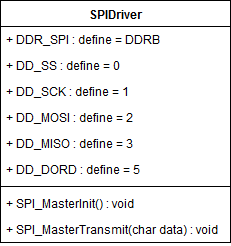
\includegraphics[width=5cm]{SPIDriverClassDiagram}
	\centering
	\caption{Class Diagram of the SPI Driver}
	\label{SpiDriverClassDiagram}
\end{figure}

Table \ref{table:SpiDriverMethodDescriptions} describes the methods of the SPIDriver.

\begin{table}[H]
	\centering
	\begin{tabular}{|c|c|}
		\hline
		\textbf{Method} & \textbf{Description} \\ \hline
		SPI\_MasterInit & \begin{tabular}[c]{@{}c@{}}This method initializes the SPI settings of the ATmega\\ to conform to what is required in order to communicate\\ with the display.\end{tabular} \\ \hline
		SPI\_MasterTransmit & \begin{tabular}[c]{@{}c@{}}This method sends data to the SPI bus, which is\\ used in order to send instructions and data to the\\ display.\end{tabular} \\ \hline
	\end{tabular}
	\caption{Method descriptions for the SPIDriver}
	\label{table:SpiDriverMethodDescriptions}
\end{table}

Since the display controller requires more logic than simply sending bytes of data via SPI, we created a Nokia5110 driver. This component makes use of the SPI driver to send instructions and data to the display. The class diagram for the Nokia5110 driver can be seen on figure \ref{Nokia5110DriverClassDiagram}.

\begin{figure}[H]
	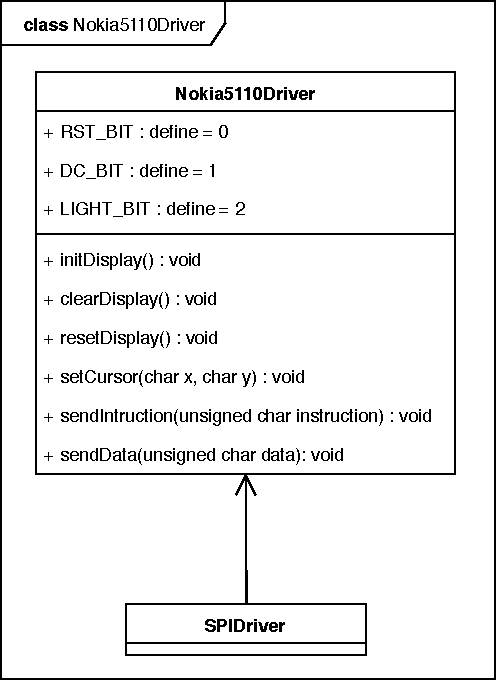
\includegraphics[width=5cm]{Nokia5110DriverClassDiagram}
	\centering
	\caption{Class Diagram of the Nokia5110 Driver}
	\label{Nokia5110DriverClassDiagram}
\end{figure}

The method descriptions of the Nokia5110 driver can be found in table \ref{Nokia5110DriverDescription}.

\begin{table}[H]
	\centering
	\begin{tabular}{ll}
		\rowcolor[HTML]{EFEFEF} 
		\textbf{Method} & \textbf{Functionality} \\
		initDisplay() & \begin{tabular}[c]{@{}l@{}}Sets the pins and ports used by\\ the display driver and SPI functionality\\ to an initialized state.\end{tabular} \\
		\rowcolor[HTML]{EFEFEF} 
		clearDisplay() & \begin{tabular}[c]{@{}l@{}}Fills the DDRAM with zeroes to clear\\ the display.\end{tabular} \\
		resetDisplay() & \begin{tabular}[c]{@{}l@{}}Resets the display by setting the reset pin \\ low and then high after a short delay.\end{tabular} \\
		\rowcolor[HTML]{EFEFEF} 
		setCursor(char x, char y) & \begin{tabular}[c]{@{}l@{}}Sets the cursor of the DDRAM to position\\ x, y.\end{tabular} \\
		sendInstruction(unsigned char) & \begin{tabular}[c]{@{}l@{}}Sets the DC pin LOW (indicating command)\\ and sends data to the display using the SPIDriver.\end{tabular} \\
		\rowcolor[HTML]{EFEFEF}
		sendData(unsigned char) & \begin{tabular}[c]{@{}l@{}}Sets the DC pin HIGH (indicating data)\\ and sends data to the display using the SPIDriver.\end{tabular}
	\end{tabular}
	\caption{Description of the methods in the Nokia5110 Driver}
	\label{Nokia5110DriverDescription}
\end{table}

When sending data to draw on the display, it is stored in the DDRAM (Display Data RAM), which is mapped to the pixels on the screen. The DDRAM is divided into 6 banks of 84 bytes. Each bit correlates to a pixel in the display, and a logical 1 turns the pixel black, while a logical 0 turns the pixel white.

Data can be placed into the DDRAM in specific spots by using x-y addressing in accordance with figure \ref{DDRAMAdressing} but is otherwise inserted using the Address Counter which is automatically incremented in accordance with the V flag (either horizontally figure \ref{HorizontalIncrement} or vertically figure \ref{VerticalIncrement}).

\begin{figure}[H]
	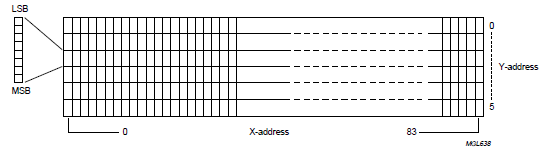
\includegraphics[width=\textwidth]{DDRAMAdressing}
	\centering
	\caption{DDRAM Addressing - Source Nokia Datasheet\cite{NokiaDisplay} page 9}
	\label{DDRAMAdressing}
\end{figure}

\begin{figure}[H]
	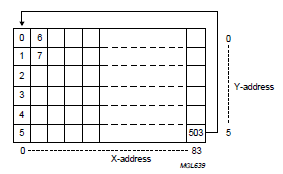
\includegraphics[]{VerticalIncrement}
	\centering
	\caption{Vertical Addressing - Source Nokia Datasheet\cite{NokiaDisplay} page 9}
	\label{VerticalIncrement}
\end{figure}

\begin{figure}[H]
	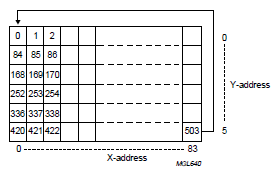
\includegraphics[]{HorizontalIncrement}
	\centering
	\caption{Horizontal Addressing - Source Nokia Datasheet\cite{NokiaDisplay} page 10}
	\label{HorizontalIncrement}
\end{figure}

In our project, we have made use of vertical addressing when filling the DDRAM.